\chapter{Topological manifolds}

\section{Some point set topology}

Some (set theoretical) conventions for the whole course:
\begin{itemize}
    \item \(A\subset B\) means A subset (not necessarily proper!) of B, i.e. \(\subset =\subseteq\)
    \item A \highlight{neighborhood} of some point \(p\in X\) means \textit{an open set \(U\subset X\) containing \(p\)}
    \item Given \(p=(p_1,\dots,p_n)\in\R^n,r>0\), \(B_r^n(p)\coloneqq \{(x_1,\dots,x_n)\mid \sum_{x_i-p_i}^2<r^2\}\). Often while \(B_s=B_s^n(0)\subset\R^n\)
\end{itemize}

\subsection{Locally Euclidean spaces}

\begin{definition*}
    A topological space \(X\) is called \dhighlight{locally Euclidean of dimension \(n\geq 0\)}, if every 
    point of \(X\) is contained in a neighborhood homeomorphic to some open subset of $\R^n$. 
\end{definition*}

\begin{remark}
    When we speak of a topological space as being \highlight{locally Euclidean}. The dimension is fixed and implicit.
\end{remark}

\begin{definition*}
    Assume that \(X\) is locally Euclidean. A \dhighlight{chart} is a pair \(U,\phi\), where \(U\subset X\),
    \(\phi:U\to\R^n\) is a homeomorphism into its image. Given \(p\in X\), we say that \(U,\phi\) is 
    \dhighlight{centered at \(p\)} if \(p\in U\) and \(\phi(p)=0\in\R^n\)
    \begin{figure}[H]
        \centering
        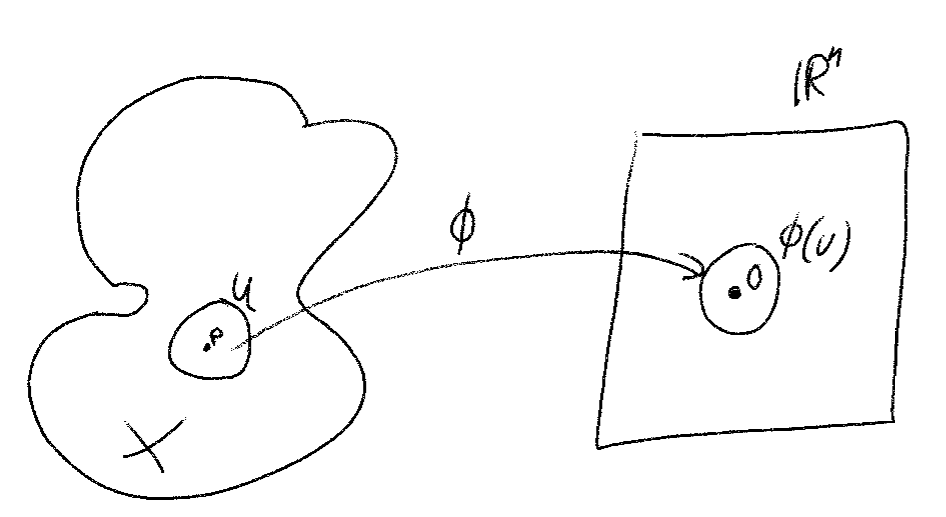
\includegraphics[width=.7\textwidth]{sketch_1_01.png}
        \caption{Sketch 1.01}
    \end{figure}
\end{definition*}

\begin{lemma}\label{lem:1.1}
    The following are equivalent (TFAE):
    \begin{itemize}
        \item \(X\) is locally Euclidean
        \item For any \(p\in X\), there is a chart \(U,\phi\) centered at \(p\) with image \(\phi(U)=B_1\)
        \item For any \(p\in X\), there is a chart \(U,\phi\) centered at \(p\) with image \(\phi(U)=\R^n\)
    \end{itemize}
\end{lemma}

\begin{proof}
    2. and 3. are equivalent, since \(B_1 \simeq \R^n\) are homeomorphic (\(B_1^n\ni x\mapsto \frac{x}{1-\Vert x\Vert}\)) % TODO: FIX 
    
    2. \(\implies \) 1. is tautological

    1. \(\implies\) 2. given \(p\in X\), since \(X\) is locally Euclidean, there exists \highlight{some} chart \(U,\phi\), \(p\in U\).
    \(psi:U\to\R^n\), homeo onto its image \(psi(U)=O\subset\R^n\). By translativity \(\R^n\ni x\mapsto x-\psi(p)\), one can assume 
    \(\psi(p)=0\in\R^n\). By scaling \(\R^n (x\mapsto \lambda x,\lambda>0)\), can assume \(B_1\subset\psi(U)\).
    Let \(U'=\psi^{-1}(B_1)\), then \((U,\psi)\) as claimed. 
\end{proof}

\subsection{Hausdorff spaces}

\begin{definition*}
    A topological space \(X\) is called Hausdorff, if given any \(p_1\neq p_2\),\(p_1,p_2\in X\), there exist neighborhoods \(p_1\in U_1,p_2\in U_2\) s.t. \(U_1\cap U_2=\emptyset\).
    \begin{figure}[H]
        \centering
        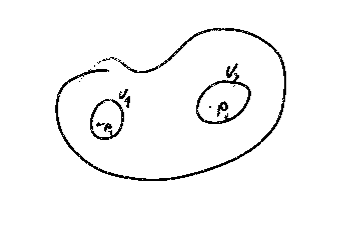
\includegraphics[width=.7\textwidth]{sketch_1_02.png}
        \caption{Sketch 1.02}
    \end{figure}
\end{definition*}

\begin{example}
    \begin{itemize}
        \item \(\R^n\)
        \item CW complexes
        \item most reasonable spaces
    \end{itemize}
\end{example}

\begin{example}[Not Hausdorff]
    \(X=\{0,1\}\), open subsets \(\emptyset,\{0\},\{0,1\}\)
\end{example}

\begin{remark}
    \(X\) is homeomorphic to \(\R/\R^*\) (quotient topology), \(R^*, (s,x\mapsto sx)\)
\end{remark}


\begin{lemma}\label{lem:1.2}
    Let \(X\) be Hausdorff. 
    \begin{enumerate}
        \item[(a)] point sets \(\{x\}\) are closed
        \item[(b)] convergent sequences have unique limits. (\(x_n\to p,x_n\to q\implies p=q\)) 
        \item[(c)] compact sets are closed 
    \end{enumerate}
\end{lemma}

\begin{proof}
    (c) \(\implies \) (a)

    For (c): Let \(K\subset X\) be compact. Want to show \(K^c\) is open. Pick \(p\in K^c\). For each 
    \(q\in K\), we can choose \(U_q\ni q, U_p\ni p: U_q\cap U_p=\emptyset\) Since K is compact, it can be covered by \(U_{q_1},\dots,U_{q_l}\). Then \(\bigcap_{i=1}^l U_{q_i}\) is oen and contains 
    \(p\), disjoint, then \(\bigcup_{i=1}^l U_{q_i}\supset K\).

    \begin{figure}[H]
        \centering
        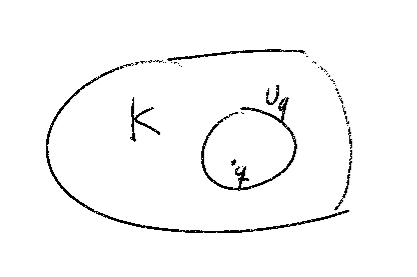
\includegraphics[width=.7\textwidth]{sketch_1_03.png}
        \caption{Sketch 1.03}
    \end{figure}

    (b) Suppose for contradiction that \(x_i\to p,x_i\to q\) and \(p\neq q\). Since \(X\) is Hausdorff, \(\exists U\ni p, O\ni q, U\cap O=\emptyset\). But for \(N>>0 x_i\in U, x_i\in O\forall i>N\)
\end{proof}


\subsection{Basis and covers}

Let \(X\) be a topological space.

\begin{definition*}
    A collection \(\cB\) of subsets of \(X\) is called a \dhighlight{basis(base)} for \(X\), if for any \(p\in X\)
    and any neighborhood \(U\ni p\), there exists an element \(\cU\in\cB\) s.t. \(p\in \cU\subset U\).
    \begin{figure}[H]
        \centering
        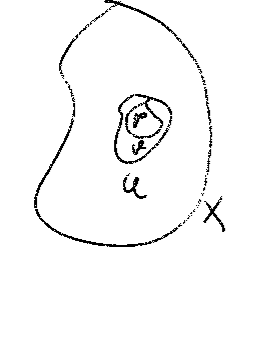
\includegraphics[width=.7\textwidth]{sketch_1_04.png}
        \caption{Sketch 1.04}
    \end{figure}
\end{definition*}


\begin{lemma}\label{lem:1.3}
    \(\cB\) is a basis for \(X\iff\) every open set of \(X\) is a union of elements of \(\cB\).
\end{lemma}

\begin{proof}
    Trivial.
\end{proof}

\begin{definition*}
    A topological space \(X\) is \dhighlight{second-countable} if it admits a countable basis.
\end{definition*}

\begin{example}
    \begin{itemize}
        \item \(\R^n\), \(\cB=\{B_s^n(p)\mid s\in \Q_+,p=(p_1,\dots,p_n)\in\Q^n\subset \R^n\}\)
    \end{itemize}
\end{example}

\begin{lemma}\label{lem:1.4}
    The property of being second-countable is closed under 
    \begin{enumerate}
        \item[(a)] subspaces
        \item[(b)] countable disjoint unions
        \item[(c)] countable products
    \end{enumerate}
\end{lemma}

\begin{remark}
    The property of being second-countable is not closed under arbitrary quotients \(q:A\to A/B\). 
    An obvious sufficient conditions is for \(q\) to be an open map. (Since it is a pushforward)\marginnote{When constructing manifolds via quotients, check that it is still second-coutable!}
\end{remark}

\begin{lemma}\label{lem:1.5}
    If \(X\) is second countable, then any open cover of \(X\) admits a countable subcover.
\end{lemma}

\begin{proof}
    Let \(\cB\) be a countable basis for \(X\). Let \(\cC\) be an open cover. 
    Let \(\tilde{\cB}\subset\cB\) be the collection of basis elements \(U\), which are contained 
    in some \(\cU\in\cC\). Observe (key!) \(\tilde{\cB}\) is a cover of \(X\). For each \(U\in\tilde{\cB}\),
    choose \(\cU_U\in\cC\) such that \(U\subset \cU_U\). Then \(\{\cU_U\}\) is a countable subcover of \(\cC\).
\end{proof}

\begin{definition*}
    Let \(X\) be a topological space. An \dhighlight{exhaustion of \(X\) by compact subsets} is a sequence \(\{K_i\}_{i\in\N}\),
    where \(K_i\subset X\) compact and \(K_i\subset \interior(K_{i+1})\) and \(\bigcup_{i=1}^\infty K_i=X\).
\end{definition*}

Recall given \(A\subset X\). \(\interior(A)\coloneqq \{x\in A\mid x \text{ in a neighborhood } U\subset A\}\).


\begin{lemma}\label{lem:1.6}
    If \(X\) is locally Euclidean, Hausdorff\footnote{not needed} and second countable. Then \(X\) admits an exhaustion by compact subsets.
\end{lemma}

\begin{proof}
    Since \(X\) is locally Euclidean, admits a basis \(\cB\) of open subsets having compact closure.\marginnote{That is take the close of \(B_{\frac{1}{2}}\subset\R^n\)}
    \begin{figure}[H]
        \centering
        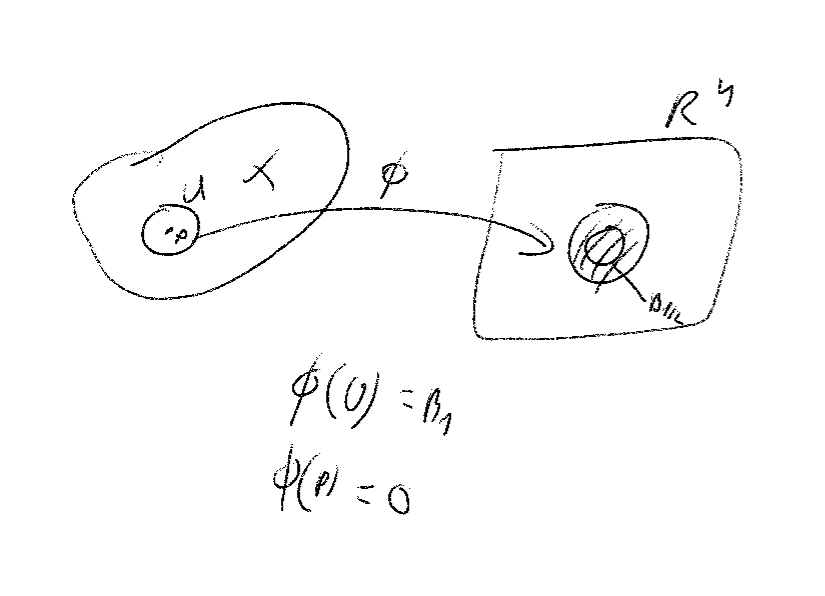
\includegraphics[width=.7\textwidth]{sketch_1_05.png}
        \caption{Sketch 1.05}
    \end{figure}
    By Lemma 1.5, one can extract a countable subcover \(\{U_i\}_{i=1}^\infty\). Set \(K_1=\overline{U_1}\).
    Assume that we already constructed \(K_1,\dots,K_k\) such that \(U_j\subset K_j\)
    and \(K_{j-1}\subset\interior(K_j),j\geq 2\). Since \(K_k\) is compact and \(K_k\subset X=\bigcup_{i=1}^\infty U_i\), then there exists some \(m_k\) such that 
    \(K_k\subset X=\bigcup_{i=1}^{m_k} U_i\) by compactness. Might as well assume that \(m_k\geq k\). Set 
    \[K_{k+1}=\overline{\bigcup_{i=1}^{m_k} U_i}=\bigcup_{i=1}^{m_k} \overline{U_i}.\] By construction \(K_{k+1}\) 
    is compact, \(K_k\subset \interior(K_{k+1})\). We get \(\{K_j\}_{j=1}^\infty\), \(U_j\subset K_j\) (because \(m_j\geq j\)) \(\implies \bigcup_{i=1}^\infty U_i=\bigcup_{i=1}^\infty K_i\)
\end{proof}
\beginlecture{02}{11.10.2024}
\subsection*{Some remarks and apologies}
\begin{itemize}
    \item Homework 01, apology for paracompactness (if this happens again, feel free to complain)
    \item Lemma \ref{lem:1.4} should be countable disjoint unions (already corrected in my notes)
    \item In lemma \ref{lem:1.6}, Hausdorff assumption not needed (already corrected in my notes)
    \item For questions about exercises, email Koen von der Dungen or your TA\footnote{tutor} directly
\end{itemize}

\begin{definition*}\label{def:local_finiteness}
    Let \(X\) be a topological space. Let \(\cC\) be a collection of subsets of \(X\). We say that \(\cC\) 
    is \dhighlight{locally finite} if for every \(x\in X\) there exists a neighborhood \(U\ni x\) such that 
    the intersection of \(U\) with all but finitely many elements of \(\cC\) is empty.
\end{definition*}

\begin{example}[Example for local finiteness]
    Take \(X=\R\), \(\cC=\{(i-1,i+1)\}_{i\in\Z}\).
    \begin{figure}[H]
        \centering
        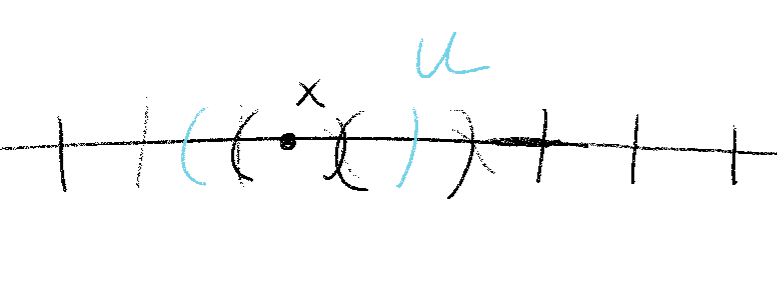
\includegraphics[width=.7\textwidth]{sketch_1_06.png}
        \caption{Sketch 1.06}
    \end{figure}
\end{example}

\begin{example}[Non-example for local finiteness]
    \(X=\R\), \(\cC=(q-1,q+1)_{q\in\Q}\)
\end{example}

\begin{definition*}\label{def:refinement}
    Let \(X\) be a topological space. Let \(\cC\) be a cover of \(X\). A cover \(\cC'\) of \(X\) is called a 
    \dhighlight{refinement of \(\cC\)}, if for all elements \(U\in\cC'\), there exists such \(V\in\cC\): \(U\subset V\).
\end{definition*}

\begin{example}[Example of Refinement]
   In the proof of lemma \ref{lem:1.5}, we showed that any open cover admits a refinement by basis elements. 
\end{example}

\begin{definition*}
    A topological space \(X\) is called \dhighlight{paracompact} if every open cover admits a locally finite refinement.
\end{definition*}

Whats up with the word \highlight{para}compact? It's like compact, but weaker! It is necessary that it only admits a locally finite refinement!

\begin{lemma}\label{lem:1.7}
    Let \(X\) be Hausdorff and suppose that \(X\) admits an exhaustion by compact subsets. Then 
    \(X\) is paracompact.In fact, we will show that given any basis \(\cB\) of \(X\), any open cover 
    admits a locally finite refinement by elements of \(\cB\).
\end{lemma}

\begin{proof}
    By assumption, \(\{K_i\}_{i\in \N}\), \(K_i\) compact, \(K_i\subset\interior(K_{i+1}),\bigcup_{i=1}^\infty K_i=X\).\marginnote{Careful! There are many definitions of exhaustion by compact sets \dots}
    Let, for  \(j\in\Z: V_j=K_{j+1}\setminus \int (K_j)\) if \(j\leq 0: K_j=\emptyset\)\footnote{He writes \(-\) for \(\setminus\)}.
    \begin{figure}[H]
        \centering
        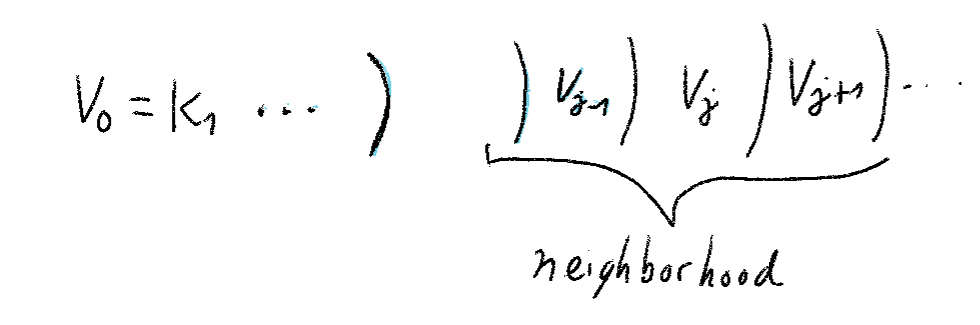
\includegraphics[width=.7\textwidth]{sketch_1_07.png}
        \caption{Sketch 1.07}
    \end{figure}
    Notice:
    \begin{itemize}
        \item \(V_j\) is compact, since we take the intersection of a compact set and a closed set. (\(\interior(K_j)^c\) is closed)
        \item \(\bigcup_{j\in \Z} V_J=X\), since \(\bigcup_{j\leq n}=\bigcup_{j\leq n+1} K_j=K_{j+1}\)
        \item The compact sets \(V_j\) are intersecting (along their boundary?) \(V_j\cap V_{j-1}=\partial K_j\coloneqq K_j\setminus\interior(K_j)\)
    \end{itemize}
    Evidently \marginnote{Here we use Hausdorffness}\(\{U_\alpha \cap \interior(K_{j+1})\cap \interior(K_{j-1})^c\}_{\alpha\in\cA}\) covers \(V_j=K_{j+1}-\setminus K_{j-1}^c\), where the \(\{U_\alpha\}_{\alpha\in\cA}\) is an open cover.
    Since \(\cB\) is a basis, we can find a refinement of this cover by basis elements. Since \(V_j\) are compact, we can extract a 
    finite subcover \(\{V_l^j\}_{l=1,\dots,k_j}\). Let's consider: \(\{V_l^j\}_{j\in Z, l=1,\dots,k_j}\). This 
    subcover works, i.e. 
    \begin{itemize}
        \item obviously a cover, since the \(V_j\) cover \(X\), obviously a refinement of \(\{U_\alpha\}\) 
        \item locally finite: given \(x\in X, x\in V_j\), hence \(x\in \interior(K_{K_{j+2}})\cap K_{j-1}^c\eqqcolon U\). If 
              \(U\cap V_l^k\), then we must have \(j-2\leq k\leq j+2\). But \(\{V_l^k\}_{j-2\leq k\leq j+2}\) is finite. \qedhere  
    \end{itemize} 
\end{proof}

\begin{corollary}\label{cor:1.8}
    If \(X\) is locally Euclidean, Hausdorff and second countable \(\implies X\) is paracompact.
\end{corollary}

\begin{proof}
    By lemma \ref{lem:1.6} (exhaustion by compact subsets) and lemma \ref{lem:1.7} \(\implies\) paracompact.
\end{proof}
\setcounter{theorem}{7}
\begin{corollary}[1.8']\label{cor:1.8'} % TODO
    Let \(X\) be Euclidean amd Hausdorff. Then \(X\) is second countable iff \(X\) has countably many components and \(X\) is paracompact.
\end{corollary}
\begin{remark}
    There are different definitions of manifolds. They differ in either forcing second countability or paracompactness. This lemma shows 
    that there only is a difference if there are uncountably many components.
\end{remark}

\begin{proof}
    Corollary \ref{cor:1.8} and the bonus homework problem from sheet 01.
\end{proof}

\begin{remark}
    Basis elements are open.
\end{remark}

\section{Topological manifolds}

\begin{definition*}
    A \dhighlight{topological \(n\)-manifold} \(M\) is a topological space with the following properties:
    \begin{enumerate}
        \item[(i)]   \(M\) is locally Euclidean (of dimension \(n\)) 
        \item[(ii)]  \(M\) is Hausdorff
        \item[(iii)] \(M\) is second countable 
    \end{enumerate}
\end{definition*}    

Morally we only really need condition (i). Why do we need the others? 
For (ii) you will not get a useful theor without it, while (iii) can be replaced by paracompactness (see corollary \ref{cor:1.8'}).

\begin{definition*}
    Let Man$^0$ be the category of topological manifolds with 
    \begin{enumerate}
        \item objects: topological manifolds 
        \item morphisms: continuous functions  
    \end{enumerate}
\end{definition*}

\begin{remark}
    \(\man0\) full subcategory of Top.
\end{remark}

\begin{remark}
    By definition, \(M,N\in\man0\), then \(M,N\) are isomorphic iff \(M,N\) are homeomorphic.
\end{remark}

\subsection{Examples of topological manifolds}

\begin{example}[Spaces isomorphic to \(R^n\)]
    \(\R^n,n\geq 0\) More generally, if \(V\) a finite dimensional \(\R\)-vector space, then \(V\)
    is a topological \(n\)-manifold.
\end{example}

\begin{example}
    Any open subset of \(\R^n\)
\end{example}

\begin{example}[Graphs]
    Let \(U\subseteq \R^n\) open, let \(f:U\to\R^n\) be a continuous function. We set 
    \[M\coloneqq\text{graph}(f)\coloneqq \{(x,y)\in U\times \R^n\mid y=f(x)\}.\]
    Then \(M\) is a manifold. The map \(M\to U\) by \((x,y)\mapsto U\) gives a global chart.
\end{example}

\begin{example}[Spheres]
    Let \(S^n\coloneqq \{x_0^2+\dots+x_n^2=1\}\subset \R^{n+1}\). Then \(S^n\) is a manifold\marginnote{Here we no longer have a global chart (for topological reasons)}.
    We define charts \[\phi_i^{\pm}:U_i^\pm = \{(x_0,\dots,x_n)\in S^n\mid \pm x_i>0\}\to B_1^n(0)\]
    by \((x_0,\dots,x_n)\mapsto (x_0,\dots,\hat{x}_i,\dots,x_n)\coloneqq (x_0,\dots,x_{i-1},x_{i+1},\dots,x_n)\)
    \begin{figure}[H]
        \centering
        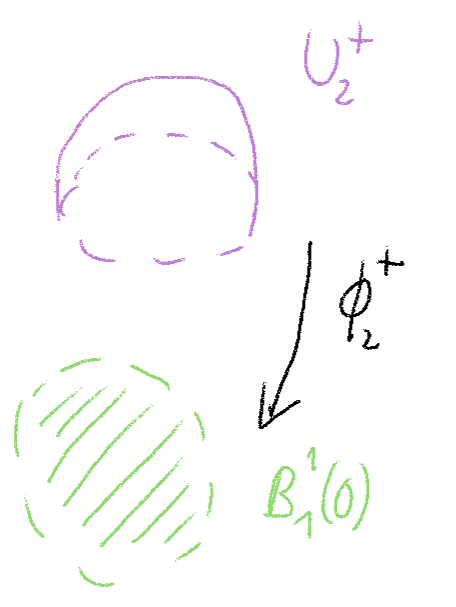
\includegraphics[width=.7\textwidth]{sketch_1_08.png}
        \caption{Sketch 1.08}
    \end{figure}
\end{example}

\begin{example}[spheres']
    Let \(C^n\coloneqq \partial([-1,1]^{n+1})=[-1,1]^{n+1}\setminus\interior([-1,1]^{n+1})\).
    Homework: \(C^n\simeq S^n\) (homeomorphic)
\end{example}

\begin{example}[\(n\)-torus]
    Let \(\Pi^n\coloneqq \R^n/\Z^n\) with the quotient topology. Then this is a manifold (exercise).
    \begin{figure}[H]
        \centering
        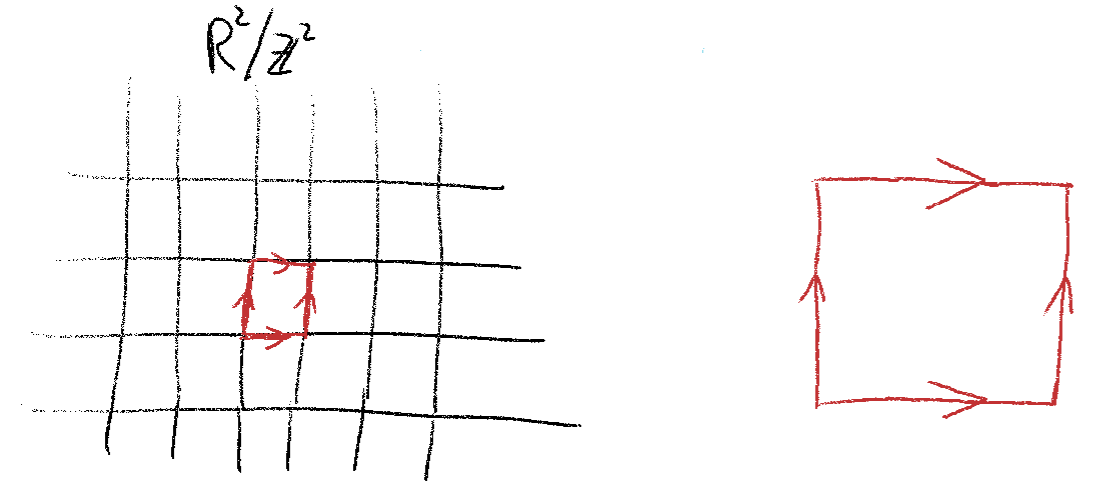
\includegraphics[width=.7\textwidth]{sketch_1_09.png}
        \caption{Sketch 1.09}
    \end{figure}
\end{example}

\begin{example}[\(\R\bP^n\coloneqq S^n/\{x\sim -x\}\)]
    \(\R\bP^n\) are also manifolds (called the real projective spaces).
\end{example}

\begin{example}[Klein bottle]
    \begin{figure}[H]
        \centering
        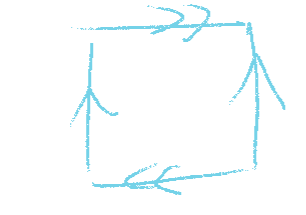
\includegraphics[width=.7\textwidth]{sketch_1_10.png}
        \caption{Sketch 1.10}
    \end{figure}
\end{example}

\begin{remark}
    \(\R\bP^2\) or generally \(\R\bP^{2n}\) and the Klein bottle are not orientable.
\end{remark}


Brief interlude: Section? %TODO

Why do we need Hausdorffness?

\begin{itemize}
    \item Back in the day (Riemann) 
    \item There is no hope to classify even 1d locally Euclidean, second-countable NOT Hausdorff spaces (See the line with two origins)
    \item With Hausdorff: Only 1d manifolds are \(\R,S^1\) (see website) 
\end{itemize}
Why do we need second countability? 
\begin{itemize}
    \item Subspaces of \(\R^n\) are second countable 
    \item We want partitions of unity (paracompactness suffices for that)
\end{itemize}

\subsection{Manifolds with boundary}

Let \(\bH^n\coloneqq \{(x_1,\dots,x_n)\in\R^n\mid x_n\geq 0\}\).
\begin{definition}
    A \dhighlight{manifold with boundary} is a topological space with the following properties:
    \begin{enumerate}
        \item[(i)] Every point has a neighborhood homeomorphic to an open subset of \(\bH^n\)
        \item[(ii)] Hausdorff
        \item[(iii)] second countable   
    \end{enumerate}
\end{definition}

Clearly every manifold is also a manifold with boundary.

\begin{example}
    \(\bH^n\) is a manifold with boundary, but not a manifold. Since for points on the boundary, there are no neighborhoods homeomorphic to Euclidean space.
\end{example}

\begin{example}
    \(S^n\cap \cH^{n+1},S^n\subset\R^{n+1}\), \([a,b],[0,\infty)\)
    \begin{figure}[H]
        \centering
        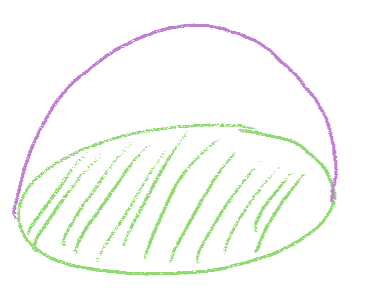
\includegraphics[width=.7\textwidth]{sketch_1_12.png}
        \caption{Sketch 1.12}
    \end{figure}
\end{example}

\begin{definition}
    If \(M\) manifold with boundary, we say \(x\) is a \dhighlight{boundary point}, if \(x\in M\setminus\interior(M)\) (i.e. it has no neighborhood homeomorphic to Euclidean space?), otherwise \(x\) is an iterior point. We let \(\partial M \coloneqq \{\text{boundary points}\}\).
\end{definition}

